\FloatBarrier
\begin{figure}[!htpd]
		\centering
		\caption{SAF}
		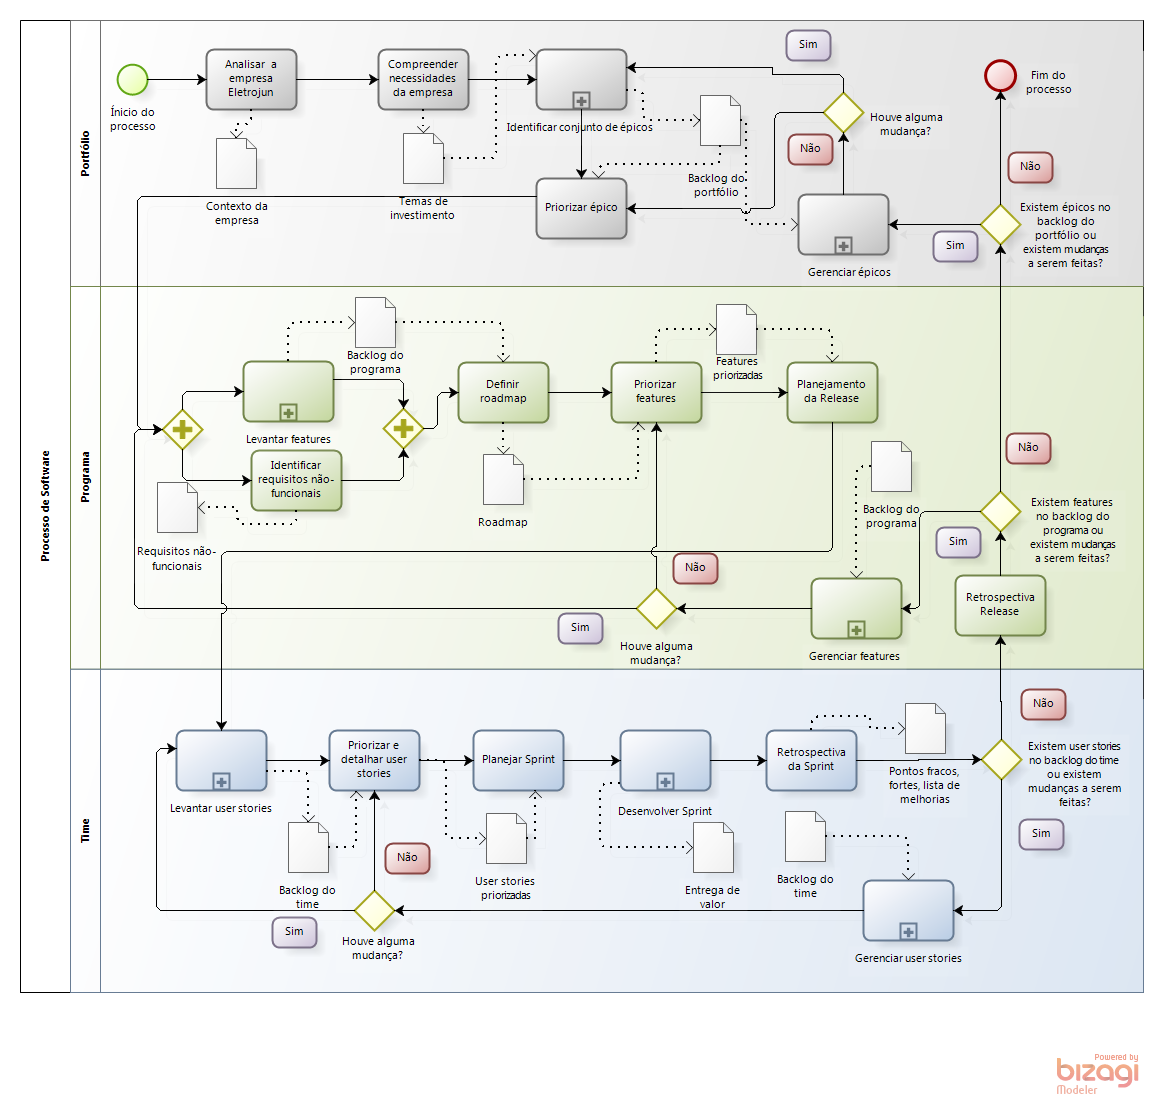
\includegraphics[scale=0.27]{figuras/Eletrojun}
		\label{img:SAF}
\end{figure}
\FloatBarrier

\section {Portifólio}

Nesta fase, todo o esforço encontra-se diretamente relacionado ao nível de negócio. Procura-se compreender o contexto do cliente, obter o conhecimento inicial do problema, identificar características e diretrizes que posteriormente  resultarão no levantamento dos Épicos.  Estes resultados serão obtidos através da efetivação das seguintes tarefas:

\begin{itemize}
\item Analisar a empresa Eletrojun
\item Compreender necessidades da empresa
\item Identificar conjunto de Épicos
\item Priorizar Épico
\item Gerenciar Épico
\end{itemize}

\begin{table}[\htp]
\centering
\caption{My caption}
\label{my-label}
\begin{tabular}{|l|l|}
\hline
ID       & 01                                                  \\ \hline
Nome     & Analisar a empresa Eletrojun.                       \\ \hline
Objetivo & Levantar informações sobre a empresa e seu negócio. \\ \hline
Entrada  &                                                     \\ \hline
Saída    & Informações sobre o contexto da empresa.            \\ \hline
\end{tabular}
\end{table}

\begin{table}[\htp]
\centering
\caption{My caption}
\label{my-label}
\begin{tabular}{|l|l|}
\hline
ID       & 02                                                  \\ \hline
Nome     & Compreender as necessidades da empresa. \\ \hline
Objetivo & Realizar entrevista com o cliente no intuito de levantar necessidades gerais \\ \hline
Entrada  &  Contexto da empresa \\ \hline
Saída    & Temas de investimento \\ \hline
\end{tabular}
\end{table}

\begin{table}[\htp]
\centering
\caption{My caption}
\label{my-label}
\begin{tabular}{|l|l|}
\hline
ID       & 03                                                 \\ \hline
Nome     & Identificar conjunto de Épicos. \\ \hline
Objetivo & Levantar conjunto de Épicos, analisando e estudando os temas de investimento.
 \\ \hline
Entrada  &  Temas de investimento. \\ \hline
Saída    & Backlog do portifólio.  \\ \hline
\end{tabular}
\end{table}

\begin{table}[\htp]
\centering
\caption{My caption}
\label{my-label}
\begin{tabular}{|l|l|}
\hline
ID       & 04                                                \\ \hline
Nome     & Priorizar Épico. \\ \hline
Objetivo & Selecionar Épico dentre o Backlog de portifólio e dar preferência ao seu desenvolvimento.
 \\ \hline
Entrada  &  Backlog do portifólio \\ \hline
Saída    & Backlog do portifólio com Épicos priorizados. \\ \hline
\end{tabular}
\end{table}

\section{Programa}

Na fase de programa, o principal objetivo encontra-se em estabelecer estratégias para elaboração da solução a ser implementada, a partir da obtenção de requisitos que atendam aos sete parâmetros de qualidade (Apendice x). Estes resultados serão obtidos através da efetivação das seguintes tarefas:

\begin{itemize}
\item Levantar Feature
\item Identificar requisitos não-funcionais
\item Definir Roadmap
\item Priorizar Features
\item Planejamento da Release
\item Gerenciar Features
zitem Planejamento da Release
\end{itemize}

\begin{table}[\htp]
\centering
\caption{My caption}
\label{my-label}
\begin{tabular}{|l|l|}
\hline
ID       & 05                                               \\ \hline
Nome     & Levantar Features. \\ \hline
Objetivo & Levantar conjunto de Features dentre o Backlog de portifólio e elaborar o Backlog de programa.
 \\ \hline
Entrada  &  Backlog do portifólio. \\ \hline
Saída    & Backlog do programa. \\ \hline
\end{tabular}
\end{table}

\begin{table}[\htp]
\centering
\caption{My caption}
\label{my-label}
\begin{tabular}{|l|l|}
\hline
ID       & 06                                               \\ \hline
Nome     & Definir Roadmap. \\ \hline
Objetivo & Planejar as entregas/releases a partir da elaboração do Roadmap .
 \\ \hline
Entrada  &  Backlog do programa. \\ \hline
Saída    & Roadmap. \\ \hline
\end{tabular}
\end{table}

\begin{table}[\htp]
\centering
\caption{My caption}
\label{my-label}
\begin{tabular}{|l|l|}
\hline
ID       & 07                                               \\ \hline
Nome     & Priorizar Features. \\ \hline
Objetivo & Selecionar Features dentre o Backlog de programa, a partir de uma análise do Roadmap,  fazer a priorização de Features.
 \\ \hline
Entrada  &  Roadmap, Backlog de programa. \\ \hline
Saída    & Features priorizadas. \\ \hline
\end{tabular}
\end{table}

\begin{table}[\htp]
\centering
\caption{My caption}
\label{my-label}
\begin{tabular}{|l|l|}
\hline
ID       & 08                                              \\ \hline
Nome     & Planejamento da Release. \\ \hline
Objetivo & Realizar o planejamento para a release, definir os pontos chaves.
 \\ \hline
Entrada  &  Features priorizadas. \\ \hline
Saída    & \\ \hline
\end{tabular}
\end{table}

\section{Time}

O nível Time abrange as tarefas a nível de implementação. Seu principal objetivo encontra-se no planejamento e implementação das funcionalidades definidas nas User Stories.  Estes resultados serão obtidos através da efetivação das seguintes tarefas:

\begin{itemize}
\item Levantar User Stories
\item Priorizar e detalhar User Stories
\item Planejar Sprints
\item Desenvolver Sprints
\item Retrospectiva da Sprint
\item Gerenciar User Stories
\end{itemize}

\begin{table}[\htp]
\centering
\caption{My caption}
\label{my-label}
\begin{tabular}{|l|l|}
\hline
ID       & 09                                             \\ \hline
Nome     & Levantar user stories. \\ \hline
Objetivo & Realizar o levantamento das histórias de usuário e com isso elaborar o backlog do time.
 \\ \hline
Entrada  &  Features priorizadas. \\ \hline
Saída    &  Backlog do time \\ \hline
\end{tabular}
\end{table}

\begin{table}[\htp]
\centering
\caption{My caption}
\label{my-label}
\begin{tabular}{|l|l|}
\hline
ID       & 10                                             \\ \hline
Nome     & Planejar Sprint. \\ \hline
Objetivo & Realizar o planejamento da sprint a ser desenvolvida, definir e distribuir tarefas.
 \\ \hline
Entrada  &  Backlog do time com User Stories priorizadas. \\ \hline
Saída    &  Kanban atualizado.\\ \hline
\end{tabular}
\end{table}

\begin{table}[\htp]
\centering
\caption{My caption}
\label{my-label}
\begin{tabular}{|l|l|}
\hline
ID       & 11                                            \\ \hline
Nome     & Desenvolver Sprint. \\ \hline
Objetivo & Executar Sprint, desenvolvendo as user stories.
 \\ \hline
Entrada  & Backlog do time atualizado, kanban. \\ \hline
Saída    &  Entrega de Valor.\\ \hline
\end{tabular}
\end{table}

\begin{table}[\htp]
\centering
\caption{My caption}
\label{my-label}
\begin{tabular}{|l|l|}
\hline
ID       & 12                                           \\ \hline
Nome     & Retrospectiva da Sprint. \\ \hline
Objetivo & Realizar reunião de retrospectiva da Sprint, de modo a discutir os pontos positivos e negativos.
 \\ \hline
Entrada  & \\ \hline
Saída    &  Lista de melhorias a serem implementadas, pontos fortes e fracos da sprint, aspectos a melhorar.\\ \hline
\end{tabular}
\end{table}
